\documentclass[]{BasiliskReportMemo}
\usepackage{AVS}
\usepackage{algorithmic}
\usepackage[boxed]{algorithm}


\newcommand{\submiterInstitute}{Autonomous Vehicle Simulation (AVS) Laboratory}

\newcommand{\ModuleName}{ThrusterForces}
\newcommand{\subject}{Algorithms to Map Desired Torque Vector onto a set of Thrusters }
\newcommand{\status}{Draft}
\newcommand{\preparer}{H. Schaub}
\newcommand{\summary}{Include a short summary of what this system engineering report is about.  Should be 300 words or less.     }


\begin{document}


\makeCover


%
%	enter the revision documentation here
%	to add more lines, copy the table entry and the \hline, and paste after the current entry.
%
\pagestyle{empty}
{\renewcommand{\arraystretch}{1.1}
\noindent
\begin{longtable}{|p{0.5in}|p{4.5in}|p{1.14in}|}
\hline
{\bfseries Rev}: & {\bfseries Change Description} & {\bfseries By} \\
\hline
v0.01 & Updated the thruster force evaluation to account for center of mass offsets & H. Schaub \\
\hline

\end{longtable}
}

\newpage
\setcounter{page}{1}
\pagestyle{fancy}

\tableofcontents
~\\ \hrule ~\\

\begin{figure}[htb]
	\centerline{
	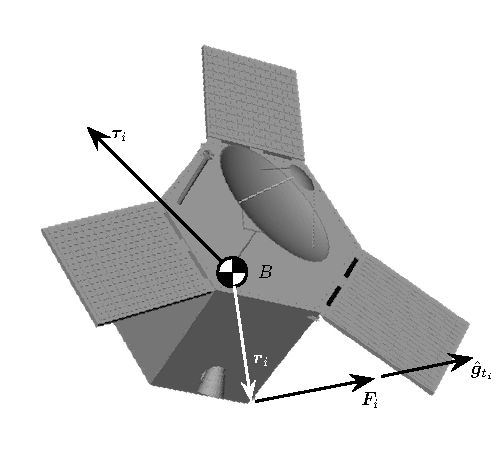
\includegraphics[]{Figures/thrusterNotation}
	}
	\caption{Illustration of the Spacecraft Thruster Notation}
	\label{fig:thruster}
\end{figure}

\section{Introduction}
This technical note describes a general algorithm that maps a desired ADCS external control torque $\bm L_{r}$ onto force commands for a cluster of thrusters.  Let $\hat{\bm b}_{j}$ be the axis about which the thrusters are to produce the desired torque.  The module can accept up to 3 orthogonal control axis $\hat{\bm b}_{j}$.  The $j^{\text{th}}$ component of $\bm L_{r}$ is given by
\begin{equation}
	L_{r,j} = \bm L_{r} \cdot \hat{\bm b}_{j}
\end{equation}�

The $i^{\text{th}}$ thruster location relative to the spacecraft point $B$ is given by $\bm r_{i}$ as illustrated in Figure~\ref{fig:thruster}.  The unit direction vector of the thruster force is $\hat{\bm g}_{t_{i}}$, while the thruster force is given by
\begin{equation}
	\label{eq:th:1}
	\bm F_{i} = F_{i} \hat{\bm g}_{t_{i}}
\end{equation}
The toque vector produced by each thruster about the body fixed point $B$ is thus
\begin{equation}
	\bm \tau_{i} = (\bm r_{i} - \bm r_{\text{COM}}) \times F_{i}  \hat{\bm g}_{t_{i}}
\end{equation}
The total torque onto the spacecraft about the body fixed axis $\hat{\bm b}_{j}$, due to a cluster of $N$ thrusters, is
\begin{equation}
	\tau_{j} = \sum_{i=1}^{N} \bm \tau_{i} \cdot \hat{\bm b}_{j}
	= \sum_{i=1}^{N}  ((\bm r_{i} - \bm r_{\text{COM}}) \times \hat{\bm g}_{t_{i}})\cdot \hat{\bm b}_{j} F_{i} = \sum_{i=1}^{N}  d_{i} F_{i}
\end{equation}
where 
\begin{equation}
	\label{eq:th1:1}
	d_{i} =   ( ( \bm r_{i} - \bm r_{\text{COM}})  \times \hat{\bm g}_{t_{i}})\cdot \hat{\bm b}_{j}
\end{equation}
In matrix form, the net spacecraft torque about the $j^{\text{th}}$ axis is written compactly as
\begin{equation}
	 \tau_{j} = \begin{bmatrix}
		 d_{1} \cdots  d_{N}
	\end{bmatrix} \begin{bmatrix}
		F_{1} \\
		\vdots \\
		F_{N}
	\end{bmatrix} = [D] \bm F
\end{equation}
where $[D]$ is a $1\times N$ matrix that maps the thruster forces $F_{i}$ to the spacecraft torque $\tau$. 


\section{Simple Thruster Force Algorithm for a Thruster Configuration with Full Torque Controllability}
The goal of the thruster force algorithm is to determine a set of thruster forces $\bm F$ such that the net force onto the spacecraft is
\begin{equation}
	\label{eq:th:2}
	\tau_{j} = \bm L_{r} \cdot \hat{\bm b}_{j} = [D]\bm F_{j}
\end{equation}
without bleeding torque onto the un-controlled axes.

The following algorithm is applied individually to control the desired torque about each $\hat{\bm b}_{j}$ axis.  
The first step to determine which  thruster forces $F_{i}$  are contributing with a positive force value.  Each thruster can only produce a positive force.  Using a minimum norm inverse of Eq.~\eqref{eq:th:2} yields
\begin{equation}
	\label{eq:th:3}
	\bm F_{j} = [D]^{T} \left( [D] [D]^{T}\right)^{-1} \bm L_{r} \cdot \hat{\bm b}_{j}
\end{equation}
This minimum norm inverse only requires inverting a $1\times 1$ matrix.  Using the SVD inverse technique, the value of this $1\times 1$ matrix is the singular value.  Thus, if this singular value is below a specified threshold $\epsilon$, the thruster configuration is not contributing to a torque about the $\hat{\bm b}_{j}$ axis.  In this case the inverse of this matrix is set to zero, and not thruster forces contribute to the desired torque about this axis.  

Note that this force stack $\bm F$ contains both positive and negative force values.  Another step is required to ensure that the thrusters can only produce positive forces.  Assume there are $M$ positive force values in $\bm F_{j}$.  The locations of these values is provided in the $N$-dimensional array $\bm t_{\text{used}}$ which contains either 0 or 1 values.  For example, consider $N=8$ and only thrusters 2 and 6 produce positive forces. In this case we find
\begin{equation}
	\bm t_{\text{used}} = \begin{bmatrix}
		0 & 1 & 0 & 0 & 0 & 1 & 0 & 0
	\end{bmatrix}
\end{equation}
This reduces the thruster force search to a subset of $M$ thrusters.  Let $\bar{\bm F}_{j}$ be a $M\times 1$ matrix of to be determined thruster forces.  The corresponding $3\times M$ mapping matrix $[\bar D]$ that projects $\bar{\bm F}_{j}$ onto a net body torque about point $B$ is defined as:
\begin{equation}
	[\bar D] = \begin{bmatrix} \bar{\bm d}_{1} & \cdots & \bar{\bm d}_{M} \end{bmatrix}
\end{equation}
with
\begin{equation}
	\bar{\bm d}_{i} = (\bm r_{i} - \bm r_{\text{COM}}) \times \hat{\bm g}_{i}
\end{equation}
The net torque due to $\bar{\bm F}_{j}$ is 
\begin{equation}
	\bar{\bm \tau}_{j} = [\bar D] \bar{\bm F}_{j}
\end{equation}

To enforce that $\bar{\bm F}_{j}$ only produces the desired torque about the $\hat{\bm b}_{j}$ axis, and not any torque about other axes, the following condition is established:
\begin{equation}
	\label{eq:thf:14}
	(\hat{\bm b}_{j} \cdot \bm L_{r}) \hat{\bm b}_{j} = [\bar D] \bar{\bm F}_{j}
\end{equation}

If the mapping matrix $[\bar D]$ has rank 3, then a minimum norm inverse can be used to determine the smallest set of thruster forces that satisfy Eq.~\eqref{eq:thf:14}.
\begin{equation}
	\bar{\bm F}_{j} = [\bar D]^{T} ([\bar D] [\bar D]^{T})^{-1}  \hat{\bm b}_{j} (\hat{\bm b}_{j} \cdot \bm L_{r})
\end{equation}
The rank condition can easily be checked by computing if the determinant of $[\bar D] [\bar D]^{T}$ is greater than zero.  If yes, a minimum norm inverse can be taken without numerical difficulties.

If the determinant of $[\bar D] [\bar D]^{T}$ is near zero, then $\bar{\bm F}_{j}$ cannot generate a general 3D torque vector.  As the spacecraft is setup with pairs of thrusters to produce the control torques, in this case the rank of $[\bar D]$ is 2, and not all body axis are influenced by $\bar{\bm F}_{j}$.  In this case the thruster forces are determined through a least-squares inverse that selects $\bar{\bm F}_{j}$ such that the controllable axes satisfy the condition in Eq.~\eqref{eq:thf:14}.  
\begin{equation}
	\bar{\bm F}_{j} = ([\bar D]^{T} [\bar D])^{-1}  [\bar D]^{T}  \hat{\bm b}_{j} (\hat{\bm b}_{j} \cdot \bm L_{r})	
\end{equation}

  
%	\begin{algorithm}
%	\caption{Logic to Enforce $F_{i}>0$ with the Simple Thruster Force Algorithm}
%	\label{alg:th:1}
%		 \begin{algorithmic}[1]
%		 	\STATE $i=1$
%			 \WHILE{$i\le 3 $}
%			 	\IF {$F_{i}>0$}
%					\STATE $F_{i} *= 2$
%				\ELSE
%					\STATE $F_{i} = 0$
%				\ENDIF
%				\STATE $i += 1$
%			 \ENDWHILE
%		 \end{algorithmic}
%	\end{algorithm}
The final step is to sum the individual $\bar{\bm F}_{j}$ thruster solutions to the yield the net set of thruster forces required to produce $\bm L_{r}$.  This is done using the  $\bm t_{\text{used}}$ matrix to determine which thrusters have non-zero contributions.  


If the thruster cluster configuration is such that pairs of thrusters produce full controllabilty, then the minimum norm solution to produce the desired $\bm L_{r}$ will also result in a thruster solution that produces a net 0 force onto the spacecraft.   Using the super-particle theorem,\cite{schaub} the total thruster force is given by
\begin{equation}
	\bm F_{T,j} = [G_{t}] \bm F_{j} =  [G_{t}] [D]^{T}([D][D])^{-1} \bm L_{r} \cdot \hat{\bm b}_{j}= \bm 0
\end{equation}
With a pure-couple thruster configuration the expression satisfies $[G_{t}] [D]^{T} = \bm 0$.



%\section{Full Thruster Force Algorithm for a General Thruster Configuration}
%Next, the case is considered where the thruster configuration is not symmetric about the center of mass, or the thruster alignments are not setup such that pure torque couples are produced.  As with the simpler algorithm described above, the positive thrust forces $F_{i}$ are determined individually to produce the desired control torque about each body axes $\hat{\bm b}_{j}$, and then these positive force solutions are summed up to obtain a final thruster force solution.
%
%The first step is again to seek the minimum norm solution to produce the desired control torque about the $\hat{\bm b}_{j}$ axis:
%\begin{equation}
%	\bm F_{j} = [D]^{T} \left( [D] [D]^{T}\right)^{-1} \bm L_{r} \cdot \hat{\bm b}_{j}
%\end{equation}
%This determines which positive thruster force solutions contribute to the desired torque.  
%
%Let $M$ be the number of thrusters that require a positive thruster force, then $\bar{\bm F}_{j}$ is the $M\times 1$ reduced set of strictly positive thruster forces, and $[\bar D]$ is  the  $3\times M$ mapping matrix with the columns $\bar {\bm d}_{i}$ defined as
%\begin{equation}
%	\bar {\bm d}_{i}=  \bm r_{i} \times \hat{\bm g}_{t_{i}}
%\end{equation}
%The reduced control torque vector $\bar{\bm L}_{r}$ is defined as
%\begin{equation}
%	\bar{\bm L}_{r} = \hat{\bm b}_{j} \left( \bm L_{r} \cdot \hat{\bm b}_{j}\right)
%\end{equation}
%This enforces that the desired torque is produced along the $\hat{\bm b}_{j}$ direction, while not impacting the torques about the other body axes.  The torque constraints are thus written as:
%\begin{equation}
%	\label{eq:th:4}
%	\bm\phi(\bar{\bm F}_{j}) = [\bar D] \bar{\bm F}_{j} - \bar{\bm L}_{r} =  0
%\end{equation}
%
%A secondary goal of the ADCS thrusters is to not produce a net force onto the spacecraft.  Using the super-particle theorem,\cite{schaub} the total thruster force is given by
%\begin{equation}
%	\bm F_{T,j} =  [\bar G_{t}] \bar{\bm F}_{j} = \bm 0
%\end{equation}
%
%Thus, the ADCS thruster force logic seeks a set of positive forces $\bar{\bm F}_{j}$ such that the net residual total force $\bm F_{T,j}$ onto the spacecraft is minimized, while the ADCS torque $\bm L_{r}$ is perfectly achieved along the $\hat{\bm b}_{j}$ direction.  The net force is minimized through the cost function
%\begin{equation}
%	J = \frac{1}{2} \bm F_{T,j}^{T} \bm F_{T,j}  = \frac{1}{2} \bar{\bm F}_{j}^{T} [\bar G_{t}]^{T}[\bar G_{t}] \bar{\bm F}_{j}
%\end{equation}
%subject to the equality constraints in Eq.~\eqref{eq:th:4}.  The augmented cost function is defined as
%\begin{equation}
%	J = \frac{1}{2} \bar{\bm F}_{j}^{T} [\bar G_{t}]^{T}[\bar G_{t}] \bar{\bm F}_{j}+ \bm\lambda^{T} ( [\bar D] \bar{\bm F}_{j} - \bar{\bm L}_{r})
%\end{equation}
%where $\bm\lambda$ is $3\times 1$ set of Lagrange multipliers.   Setting its gradient equal to zero yields the following necessary conditions:
%\begin{equation}
%	\begin{bmatrix}
%		\bar G_{t}^{T} \bar G_{t} & \bar D^{T} \\
%		\bar D & \bm 0_{3\times 3}
%	\end{bmatrix} \begin{bmatrix}
%		\bar {\bm F}_{j} \\
%		 \bm\lambda
%	\end{bmatrix} = \begin{bmatrix}
%			\bm 0_{M\times 1} \\
%		\bar{\bm L}_{r} 
%	\end{bmatrix}
%\end{equation}
%The square matrix on the left hand side is of dimension $M+3$.  
%This system of equations must be solved using a robust matrix inverse, such as the SVD based inverse. Depending on the thruster alignment and availability, this matrix will not always be of full rank.  Assume some thrusters are off-line, as the ADCS torque requirement is provided as an equality constraint, the thrusters will produce the desired $\bm L_{r}$ vector, even if the net force is non-zero.  
%
%This process is now repeated for the remaining two body axes directions.  The final set of thruster forces is obtained through a summation of all the sub-results.
%\begin{equation}
%	\bm F = \sum_{j=1}^{3} \bm F_{j}
%\end{equation}


\section{Module Parameters}
\subsection{$\epsilon$ Parameter}
The minimum norm inverse in Eq.~\eqref{eq:th:3} requires a non-zero value of $[D][D]^{T}$.  For this setup, this matrix is a scalar value
\begin{equation}
	D_{2} = [D][D]^{T}
\end{equation}
The $d_{i}$ matrix components are given in Eq.~\eqref{eq:th1:1}.  Using the robust SVD inverse technique, $D_{2} > \epsilon$, then the $1/D_{2}$ math is evaluated as normal.  However, if $D_{2}<\epsilon$, then the inverse $1/D_{2}$ is set to zero.  In the latter case there is no control authority about the current axis of interest.  To set this epsilon parameter, not the definition of the $[D]$ matrix components $d_{i} = (\bm r_{i} \times \hat{\bm g}_{t_{i}}) \cdot \hat{\bm b}_{j}$. Note that $\bm r_{i} \times \hat{\bm g}_{t_{i}}$ is a scaled axis along which the $i^{\text{th}}$ thruster can produce a torque.  The value $d_{i}$ will be near zero if the dot product of this axis with the current control axis $\hat{\bm b}_{j}$ is small.  

To determine an appropriate $\epsilon$ value, let $\alpha$ be the minimum desired angle to avoid the control axis $\hat{\bm b}_{j}$ and the scaled thruster torque axis $\bm r_{i} \times \hat{\bm g}_{t_{i}}$ being orthogonal.  If $\bar r$ is a mean distance of the thrusters to the spacecraft center of mass, then the $d_{i}$ values must satisfy
\begin{equation}
	\frac{d_{i}}{\bar r} > \cos(90\dg - \alpha) = \sin\alpha
\end{equation}
Thus, to estimate a good value of $\epsilon$, the following formula can be used
\begin{equation}
	\epsilon \approx d_{i}^{2} = \sin^{2}\!\alpha \ \bar{r}^{2}
\end{equation}
For example, if $\bar{r} = 1.3$ meters, and we want $\alpha$ to be at least 1$\dg$, then we would set $\epsilon = 0.000515$.

\subsection{$[B]$ matrix}
The module requires control control axis matrix $[B]$ to be defined.  Up to 3 orthogonal control axes can be selected.  Not that in python the matrix is given in a 1D form by defining {\tt controlAxes\_B}.  Thus, the $\hat{\bm b}_{j}$ axes are concatenated to produce the input matrix $[B]$. 

\bibliographystyle{unsrt}
\bibliography{references}



\end{document}
